\documentclass[12pt,a4paper]{article}
\usepackage[utf8]{inputenc}
\usepackage[a4paper,vmargin={17mm,20mm},hmargin={20mm,10mm}]{geometry}
\usepackage{amsmath}
\usepackage{amssymb}
\usepackage{mathtools}
\usepackage{gensymb}
\usepackage{enumitem}
\usepackage{graphicx}
\usepackage{scrextend}
\usepackage{blindtext}
\usepackage{caption}
\usepackage{url}
\usepackage{subcaption}
\usepackage{circuitikz}
\usepackage{listings}
\usepackage{color}
\usepackage{hyperref}
\usepackage{subcaption}
 
\definecolor{codegreen}{rgb}{0,0.6,0}
\definecolor{codegray}{rgb}{0.5,0.5,0.5}
\definecolor{codepurple}{rgb}{0.58,0,0.82}
\definecolor{backcolour}{rgb}{0.95,0.95,0.92}
 
\lstdefinestyle{mystyle}{
    backgroundcolor=\color{backcolour},   
    commentstyle=\color{codegreen},
    keywordstyle=\color{magenta},
    numberstyle=\tiny\color{codegray},
    stringstyle=\color{codepurple},
    basicstyle=\footnotesize,
    breakatwhitespace=false,         
    breaklines=true,                 
    captionpos=b,                    
    keepspaces=true,                 
    numbers=left,                    
    numbersep=5pt,                  
    showspaces=false,                
    showstringspaces=false,
    showtabs=false,                  
    tabsize=2
}
 
\lstset{style=mystyle}
 

\DeclarePairedDelimiter\floor{\lfloor}{\rfloor}
\title{AI lab Project Report}
\date{\today}
\author{By Alessandro Vecchi}
\sloppy
\begin{document}
\title{\textbf{AI lab Project Report}}
\author{Alessandro Vecchi and Francesco Danese}
\date{\today}
\maketitle

%this is the tenth question

\begin{abstract}

\begin{addmargin}[3em]{1em}
\centering
Throughout the AI Lab course we have learnt many Computer Vision and Deep Learning concepts and we applied almost all of them directly or indirectly in our final lab project. Additionally, having taken away a lot from this course, we aimed to make a project that would challenge us academically and intellectually. For our final project, we made an autonomous lane-following car, built by us, that is also able to stop in front of STOP signals and detect if there are pedestrian in the path.
\end{addmargin}

\end{abstract}

\section{Introduction}
%starting off with the answer
\subsection{Problem Statement}
\begin{large}
It's been quite a journey. We decided to tackle the problem of building from start to finish a self-driving car with Raspberry Pi 4 with a lane following algorithm that doesn't rely on deep learning, but only on a pipeline of various Image Processing techniques. It's been an awesome project, even if we spent a lot of time doing it we enjoyed every part of it. The feeling of succedingly building a self-driving car is unbearable, not mentioning that it can stop and restart at the STOP signal flawlessly. \\
Originally, we wanted to implement also a lane following algorithm with neural networks and to perform semaphore recognition with a 3D printed semaphore, but we underestimated the amount of time required for this huge project and the rest of the time was spent in internships and for studying the other 4 exams of the semester. But still we manage to complete a lot of tasks and we couldn't be any happier! \\
Next year we could improve the project during the Deep Learning course by creating a neural network solution to the problem and add vocal commands and speech processing tasks during the NLP course. There is still a lot to be done and we can't wait to go further in learning but, for now, let's settle and fully understand the topics of this course!
\subsection{Engineering Design Tasks}
As engineers, we take on the task of designing a new device with a unique approach which highlights our skills as effective problem solvers. Essentially, to design a semi-autonomous vehicle for our final project we followed 4 essential steps which were necessary in coming up with a solution to the problem statement. 

\begin{itemize}
\item[1] We evaluated the challenge by defining goals and the constraints in the problem.
\item[2] We researched by reading our helpful Lab modules and procedures to design many possible solutions.
\item[3] After coming up with these solutions, we chose the best possible solution that solved the problem in the most efficient way for our prototype.
\item[4] Testing the solution is the last step in the engineering design algorithm and hence, we performed various tests on the vehicle, tweaked it to make it more functional and tested it on many test cases as necessary. 
\end{itemize}
\newpage

\section{Building the Robot}


\subsection{Components}

The main idea was to build a small car that was able to see. To achieve all the tasks needed for such a robot, we made the following shopping list: 
\begin{itemize}
  \item 3 big batteries for powering the motors (3.7V each one).
  \item 1 Powerbank to power the Raspberry.
  \item 4 DC motors and wheels.
  \item A two-level chassis made of plastic plates to accomodate all the devices.
  \item 1 Raspberry-Pi-4 as computational unit, basically, the computer.
  \item 1 L298 h-bridge driver, wired to the batteries and the computer, that takes signals from the Raspberry Output pins and give the right amount of energy to the motors.
  \item 1 Camera of 8MP compatible with the Pi and a Wide-Angle lens to retain a more spreaded view.
  \item A 3D-printed arm to hold the camera lifted up.
  \item A bunch of wirings, double sided tape, screws and bolts.
\end{itemize}
Let's see how those components look: 

\begin{figure}[hb]
  \centering
  \begin{subfigure}{0.2\textwidth}
    \centering
    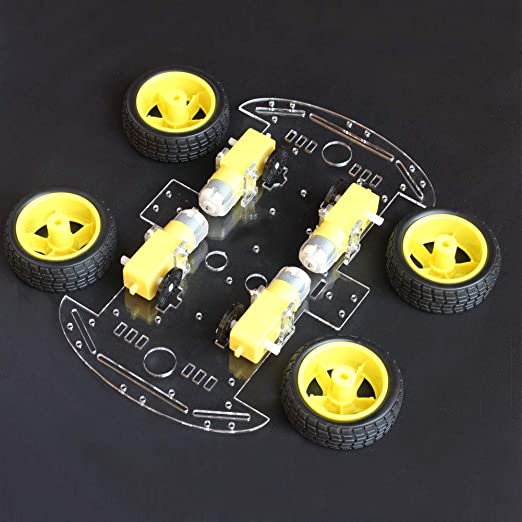
\includegraphics[width = \textwidth]{images/Chassis.jpg}
    \caption{Wheels, motors and chassis}
    \label{fig:left}
    \end{subfigure}
  \begin{subfigure}{0.2\textwidth}
    \centering
    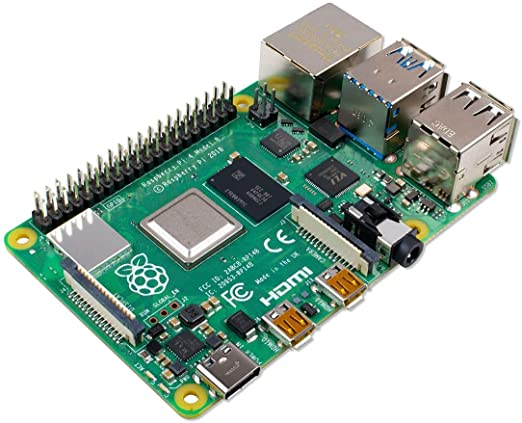
\includegraphics[width = \textwidth]{images/rasp.jpg}
    \caption{Raspberry Pi 4}
    \label{fig:right}
    \end{subfigure}
  \begin{subfigure}{0.2\textwidth}
    \centering
    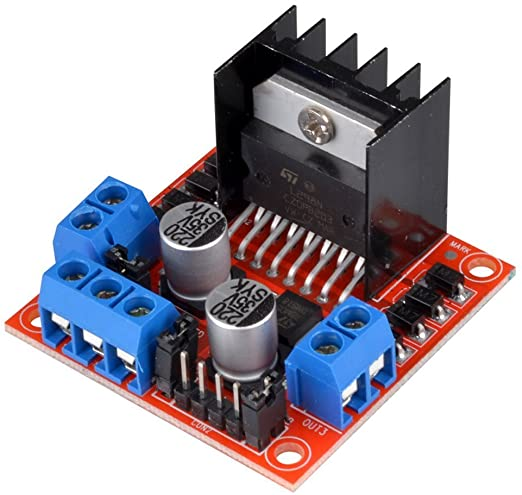
\includegraphics[width = \textwidth]{images/bridge.jpg}
    \caption{L298n Motor Driver}
    \label{fig:right}
    \end{subfigure}
  \begin{subfigure}{0.2\textwidth}
    \centering
    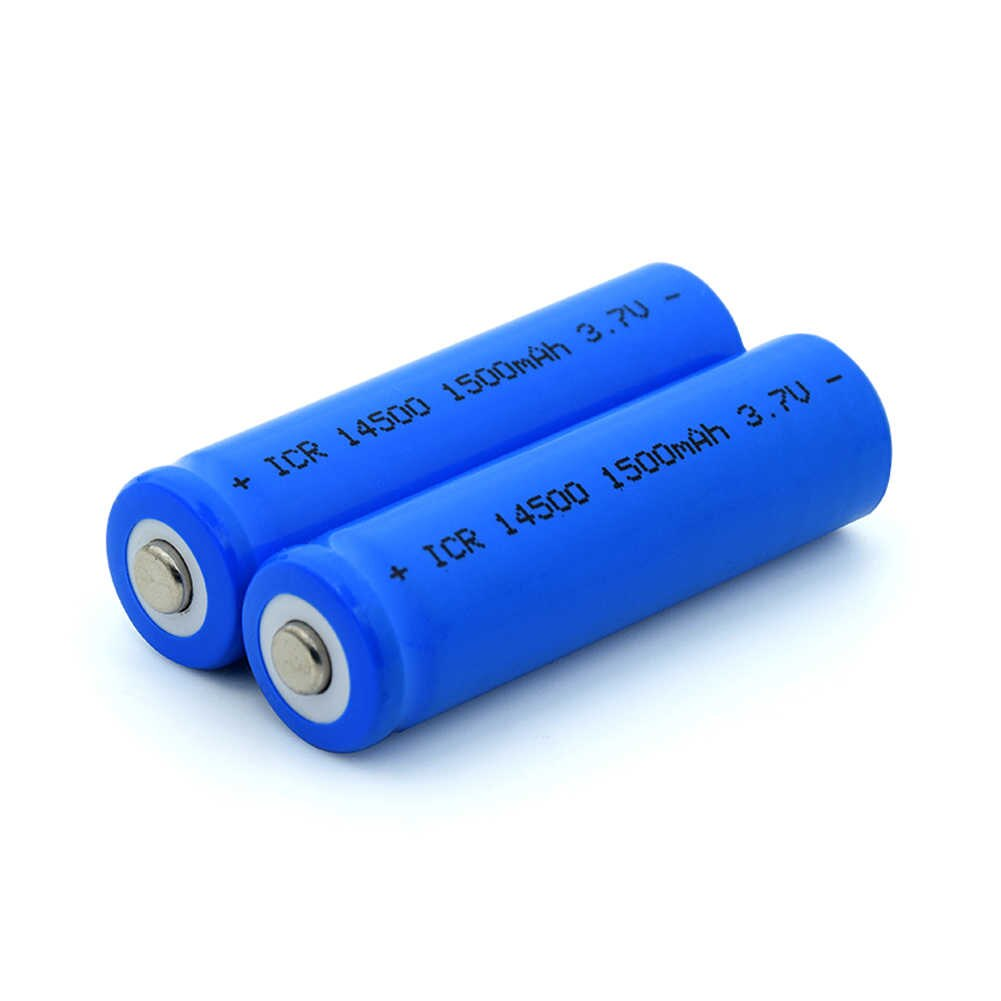
\includegraphics[width = \textwidth]{images/batterie.jpg}
    \caption{Motor's batteries}
    \label{fig:right}
    \end{subfigure}
  \begin{subfigure}{0.2\textwidth}
    \centering
    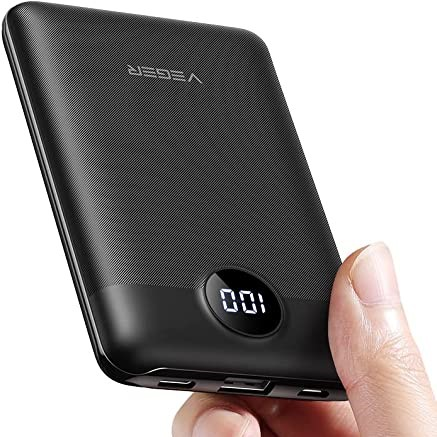
\includegraphics[width = \textwidth]{images/powerbank.jpg}
    \caption{Powerbank}
    \label{fig:right}
    \end{subfigure}
  \begin{subfigure}{0.2\textwidth}
    \centering
    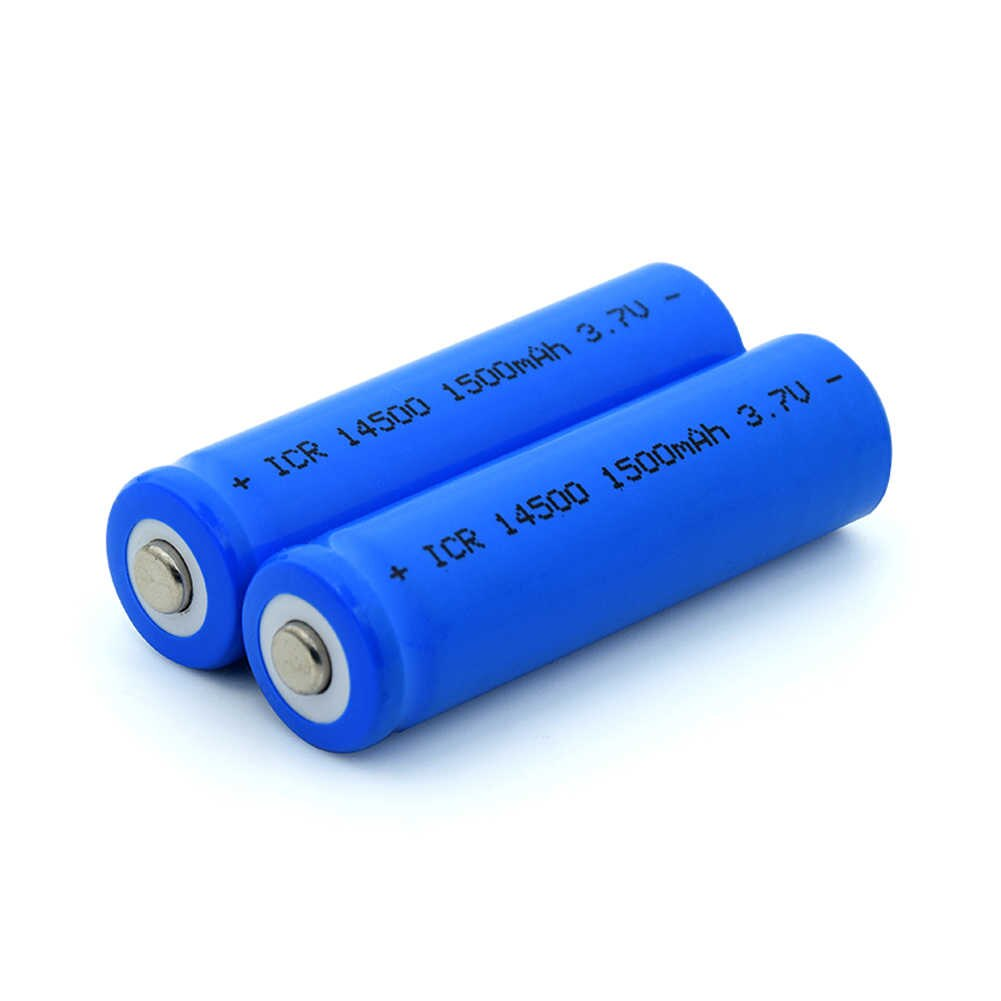
\includegraphics[width = \textwidth]{images/batterie.jpg}
    \caption{Motor's batteries}
    \label{fig:right}
    \end{subfigure}
  \label{fig:combined}
\end{figure}

\subsection{Assembling all the parts}
Now it's time to give a sense to this pile of stuff, and mount all the components together. On the bottom level of the robot will be located the two power sources, batteries and powerbank, along with the l298n driver. On the top level will sit the Raspberry and the camera mounted on the 3D-printed support. Here's a picture of the complete robot:
\begin{figure}[hb]
\centering
\begin{subfigure}{0.4\textwidth}
  \centering
  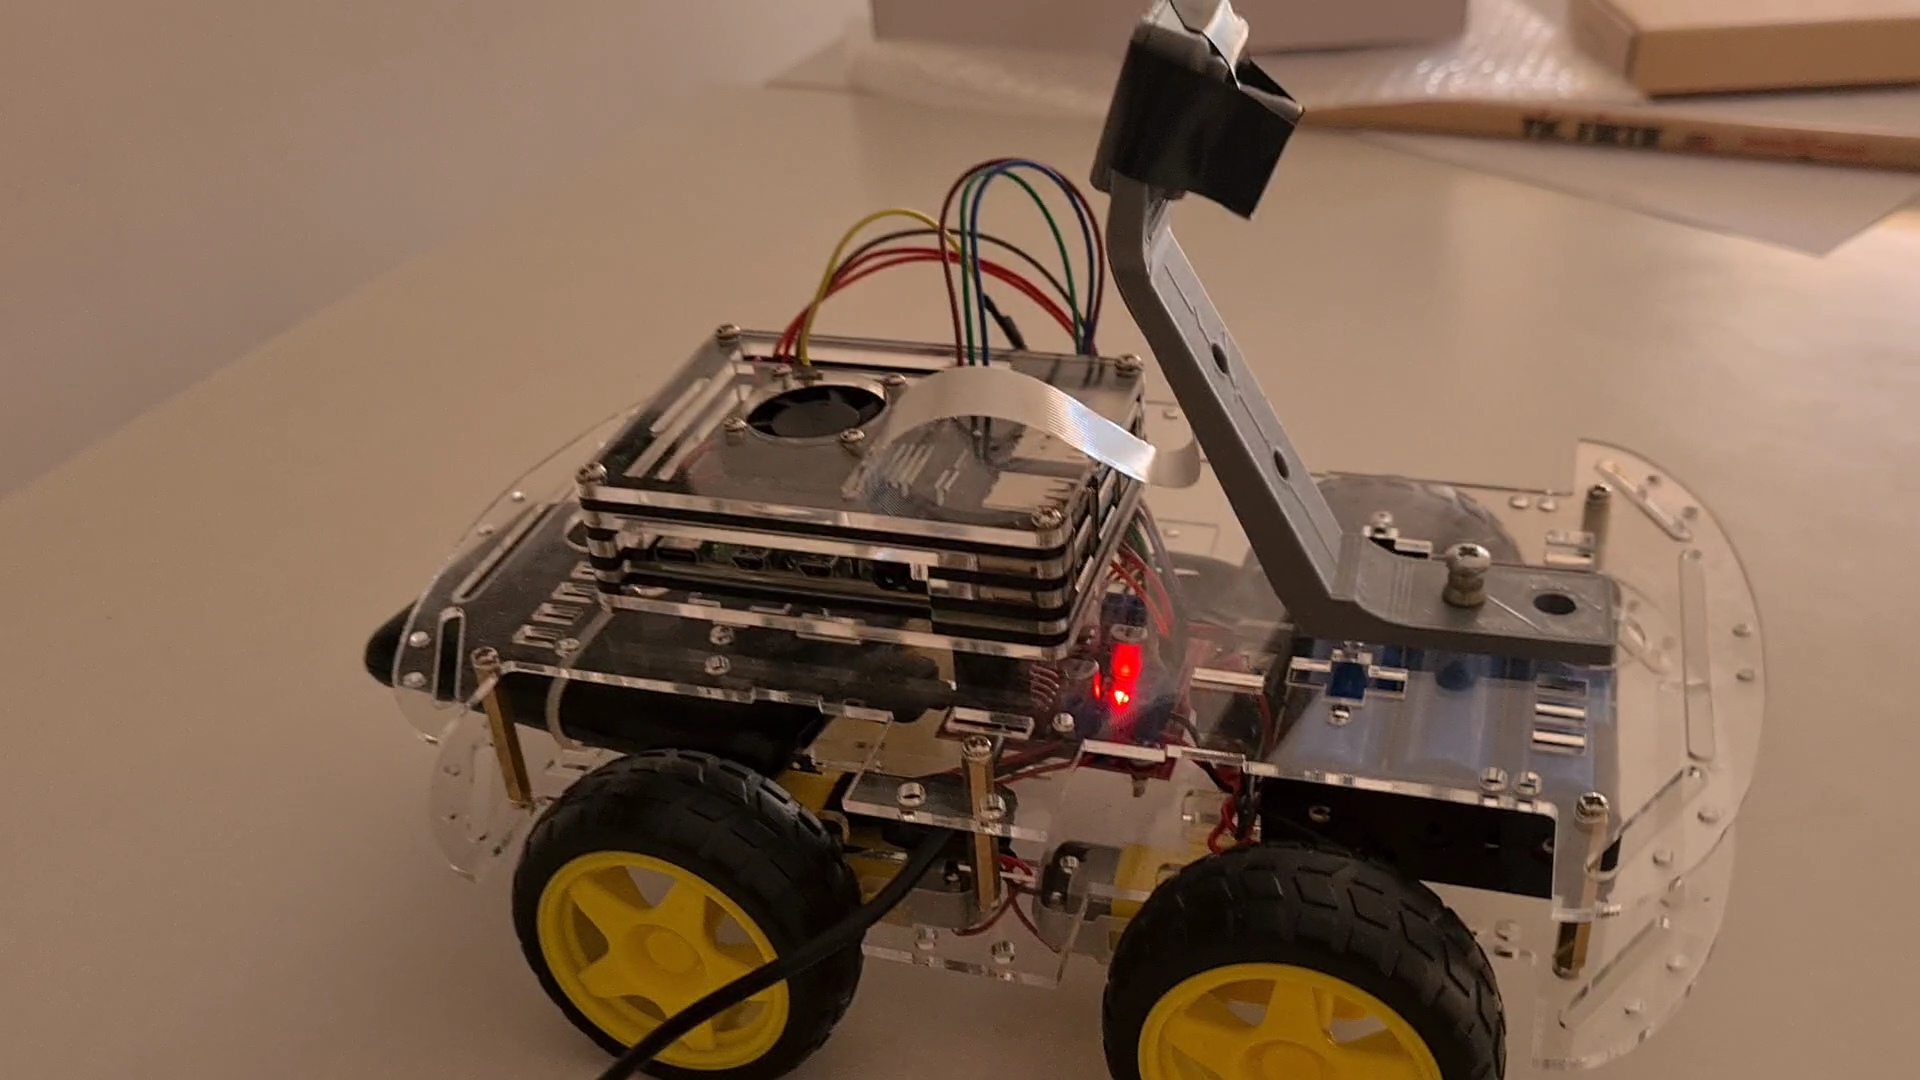
\includegraphics[width = \textwidth]{images/car1.jpg}
  \caption{Powerbank}
  \label{fig:right}
  \end{subfigure}
\begin{subfigure}{0.4\textwidth}
  \centering
  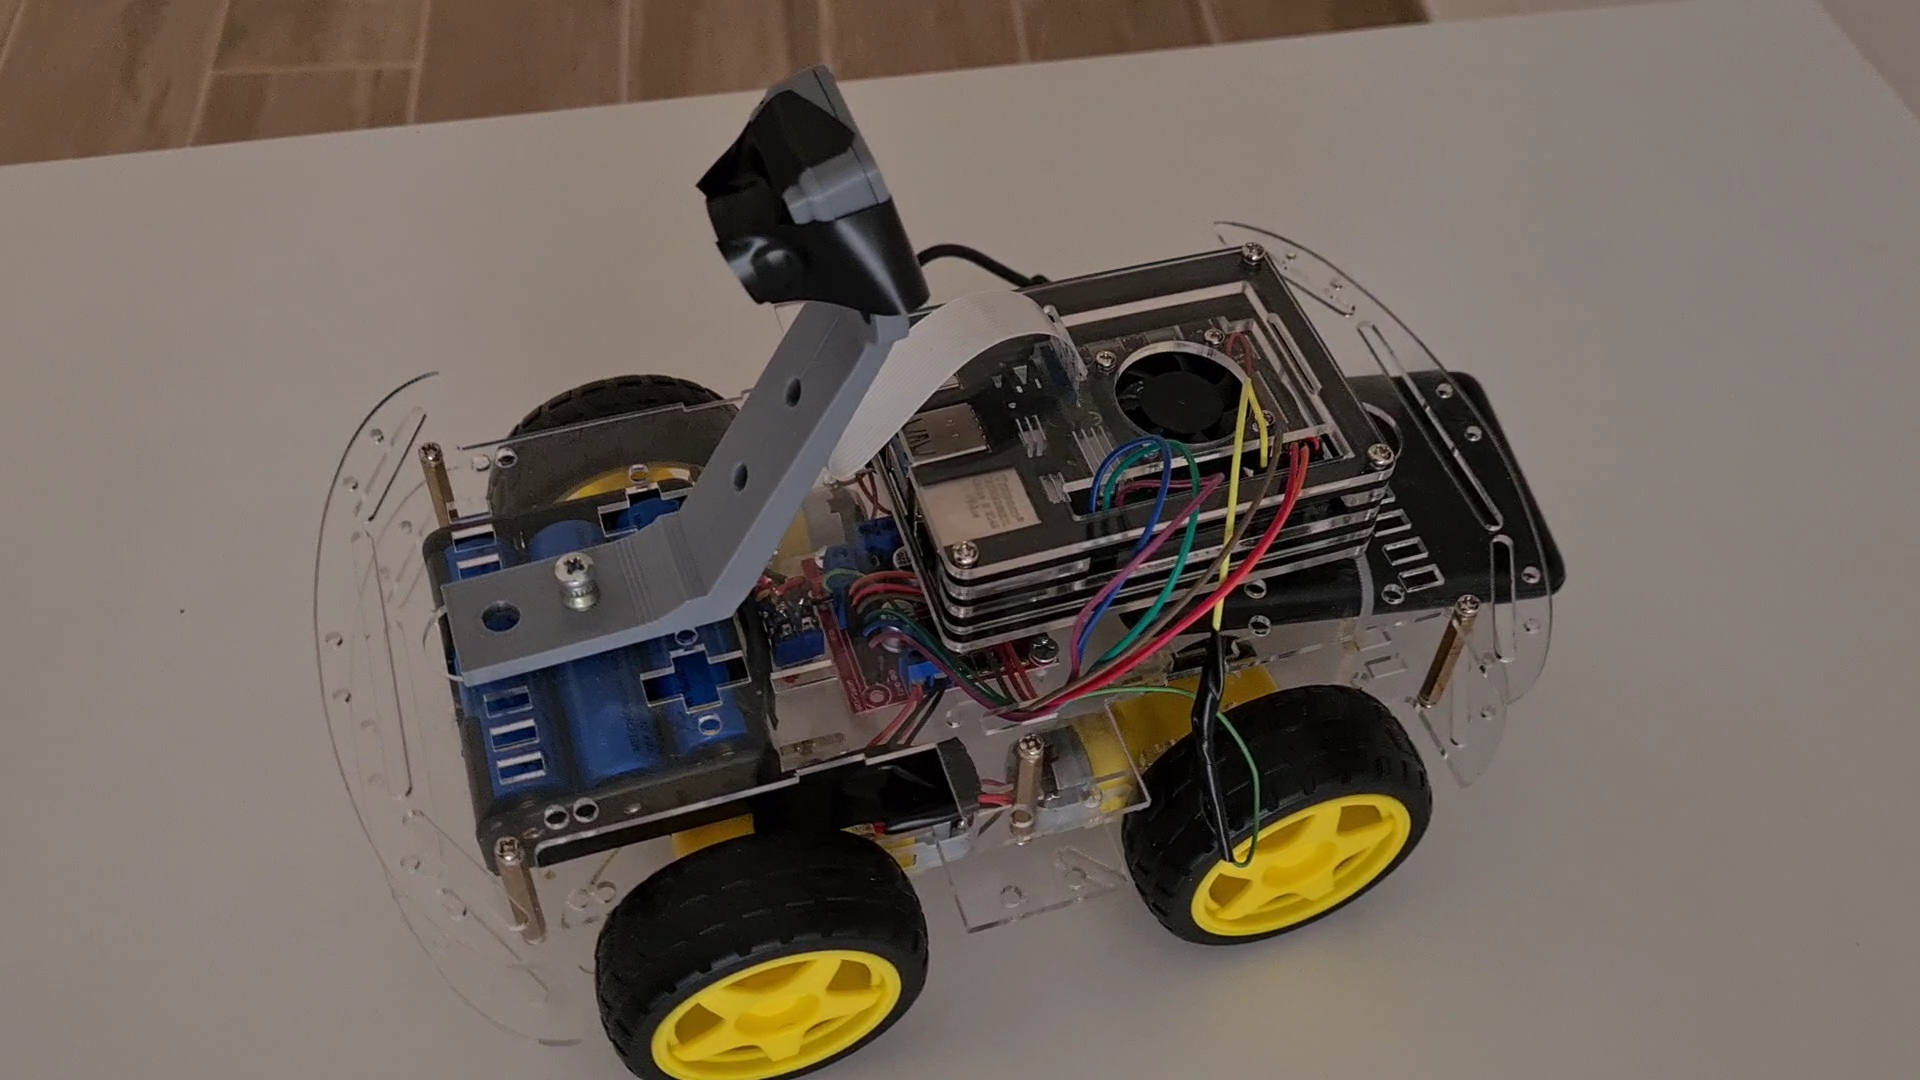
\includegraphics[width = \textwidth]{images/car2.jpg}
  \caption{Powerbank}
  \label{fig:right}
  \end{subfigure}
\end{figure}

\subsection{Resistors}

Resistors are a chief electrical component in circuits - they are used to reduce current flow and at the same time maintain low voltage levels  to prevent short circuits and provide the required current flow in simple circuits. In our project we have used these resistors in several points in the circuit accordingly. The resistance values used in our circuits are - $~~~~~ADD ~~R~~ VALUES ~~HERE~~~~$\\


\subsection{Capacitors}

Capacitors are also an essential part of electronic circuits. It's formally defined as a passive two-terminal electrical component used to store electrical energy temporarily in an electric field. We used capacitors in our project in places according to a pre-designed circuit. (ECE 110 gives preliminary circuit component study) The capacitance values used in our circuit are - $~~~~~ADD ~~C~~ VALUES ~~HERE~~~~$

\subsection{Microphone}

A microphone is formally defined as an acoustic-to-electric transducer or simply, a sensor that can convert audio signals to electric signals. In our project we used the microphone to detect a clap - essentially a large pressure variation - from its environment and move or stop the vehicle. To control this, we used our own code using the Arduino. (\textit{code posted below})
\subsection{RedBot Sensors}

The RedBot sensor works by detecting reflected light coming from its own Infrared LED. By measuring the amount of reflected light it can detect transitions from dark to light lines and even objects directly in front of it. The sensor has a 3-pin head which connects directly to the Arduino using female-female jumper cables. For our project, we had to write code compatible with our project requirements and hence used the RedBot library to detect lines or objects. \\

An image of the sensor and the data-readings (the characteristic) as a function of its distance from white paper is attached below. 

\begin{figure} [hbp]
\centering
  \begin{subfigure}[b]{0.4\textwidth}
  \centering
  \captionsetup{justification=centering}
    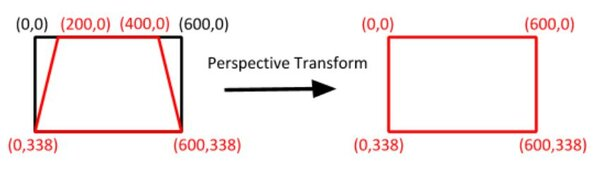
\includegraphics[width=4cm, height = 6cm]{images/perspective_transform.jpg}
    \caption{Image of the sensor \\Source \protect\url{http://bit.ly/1LFJ5Xr}}
   
  \end{subfigure}
  \hspace{1cm}
  \begin{subfigure}[b]{0.4\textwidth}
  \centering
  \captionsetup{justification=centering}
    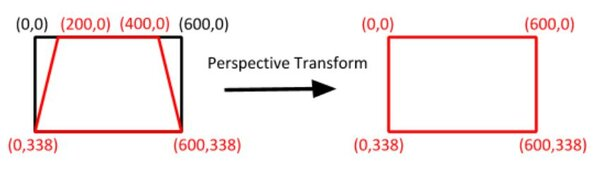
\includegraphics[width=\textwidth, height = 6cm]{images/perspective_transform.jpg}
    \caption{Characterization of the sensor \\(generated with Octave)}
    
  \end{subfigure}
  \caption{RedBot sensor diagram and Characterization}
\end{figure}

\section{Lane detection with Image processing}

The main idea here is to find the path using color detection and then iteratively moving the car at the center of the road.\\
In order to reach this goal we are going to divide the task in 5 different steps:

\begin{itemize}
  \item[1] Thresholding the frames;
  \item[2] Warping the perspective;
  \item[3] Finding the center of the road;
  \item[4] Understanding how to curve;
  \item[5] Hardware implementation.
  \end{itemize}

\begin{figure}[hbp]
\centering
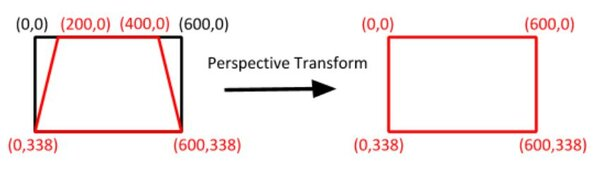
\includegraphics[width=0.4\textwidth, height = 4cm]{images/perspective_transform.jpg}
\caption{\label{fig:5}Test track for the vehicle with curved corners\\Source: \protect\url{http://bit.ly/1PTRAGf}}
\end{figure}

\subsection{Thresholding}
Recall that our "street" consists of plain A4 white paper, so a cool way to find the path is to apply simple thresholding to each frame.\\
The original way we were doing it was by converting the BGR image to an HSV one. The reason is that since the hue channel models the color type, it is very useful to segment the road based on its color and we could tune the saturation to express the "whiteness" of our image. Thus to select our path we selected a range of white-ish pixels using trackbars and set them to 255, while all the others were set to 0. However, we then discovered that this method was very dependent to the lightning conditions since it was a static way of determine the threshold and so we had to change the thresholding section a little bit. We tried a lot of methods and the ones that worked best were Otsu's thresholding and a conversion to the HSL color space to remove the very bright portions of the frame.\\
In order to achieve this we will use the \href{https://docs.opencv.org/3.4/da/d97/tutorial_threshold_inRange.html}{inRange} function of OpenCV and to select the right thresholds we use a slightly modified version of the color picker offered by the link above.

\begin{figure} [!htb]
  \centering
    \begin{subfigure}[b]{0.4\textwidth}
    \centering
    \captionsetup{justification=centering}
      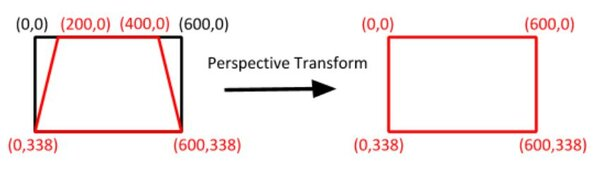
\includegraphics[width=4cm, height = 6cm]{images/perspective_transform.jpg}
      \caption{How we see the path}
      
    \end{subfigure}
    \hspace{1cm}
    \begin{subfigure}[b]{0.4\textwidth}
    \centering
    \captionsetup{justification=centering}
      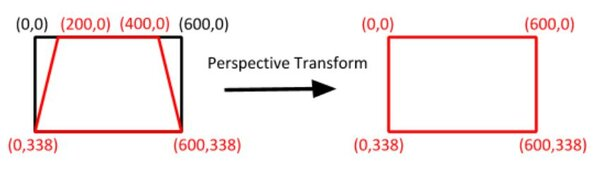
\includegraphics[width=\textwidth, height = 6cm]{images/perspective_transform.jpg}
      \caption{Thresholded path \\}
      
    \end{subfigure}
  \end{figure}

\subsection{Warping}
Recall that one of our goals is to determine the radius of curvature of the road lane, in order to be able to perform the curve. \\
The problem is that the camera perspective is not an accurate representation of what is going on in the real world. From its point of view, the lane lines form a trapezoid-like shape. We can't compute the radius of curvature of the road because the lane width seems converging to a point, as you can see from this example:\\

\begin{figure} [!htb]
\centering
\captionsetup{justification=centering}
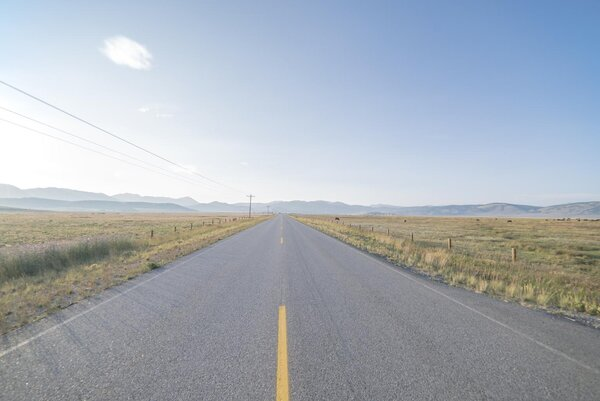
\includegraphics[width=8cm]{images/road_endless_straight_vanishing.jpg}
\caption{Camera's perspective}
\end{figure}

To fix this, we can apply a perspective transformation that warp the camera's perspective into a birds-eye view perspective.

\begin{figure} [!hb]
  \centering
  \captionsetup{justification=centering}
  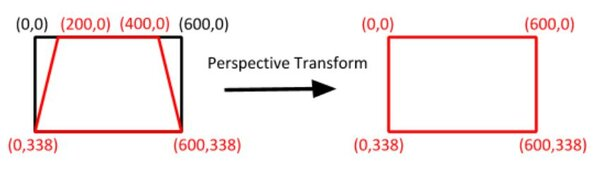
\includegraphics{images/perspective_transform.jpg}
  \caption{Perspective transform}
  \end{figure}

To do this we need to identify the region of interest, defined by the four corner of our trapezoid. In this way we can concentrate only on the parts of the image we're interested in, namely the ones immediately in front of the car. We determined these points manually, by experimenting with different values on the trackbars. Now we can obtain the transformation matrix using the built-in "getPerspectiveTransform"" and then we can get the warped image with the "warpPerspective" method.

\begin{figure} [!hbp]
  \centering
    \begin{subfigure}[b]{0.3\textwidth}
    \centering
    \captionsetup{justification=centering}
      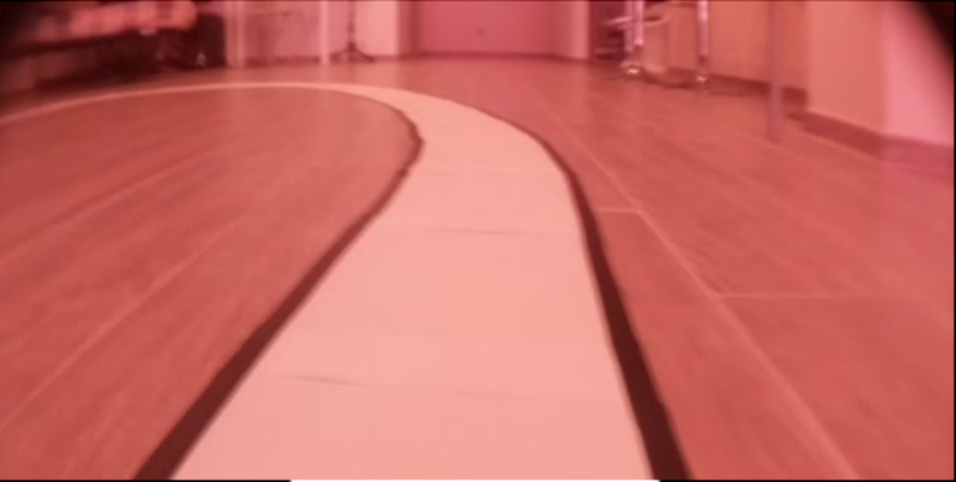
\includegraphics[width=\textwidth]{images/camera_perspective.png}
      \caption{Road in perspective}
      
    \end{subfigure}
    \hspace{0.1cm}
    \begin{subfigure}[b]{0.3\textwidth}
    \centering
    \captionsetup{justification=centering}
      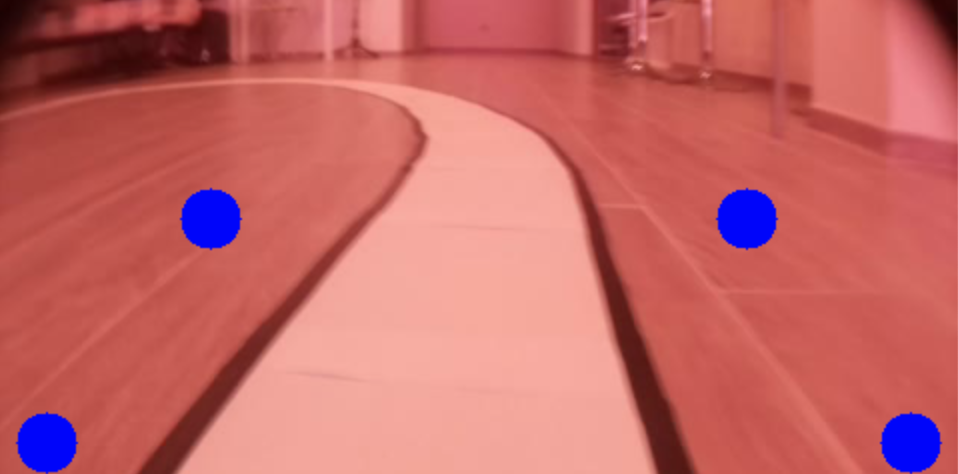
\includegraphics[width=\textwidth]{images/points_warp.png}
      \caption{Points for tuning the warping \\}
      
    \end{subfigure}
    \hspace{0.1cm}
    \begin{subfigure}[b]{0.3\textwidth}
    \centering
    \captionsetup{justification=centering}
      
\includegraphics[width=\textwidth]{images/birds_eye_view.png}
      \caption{Bird eye view \\}
      
    \end{subfigure}
  \end{figure}

\subsection{Centering}
In order for our supercar to move smoothly and to detect curves properly, we have to make it move at the center of the road. But how do we find the center? \\
Well, it turns out that is rather easy. Ideally, we have a black image and a white road seen from above. A logical way of finding the center of the road is to consider the part of the image that is immediately near the camera and find the average column between those that have a relevant amount of white pixels.

\begin{figure} [!htb]
  \centering
  \captionsetup{justification=centering}
  % \includegraphics{lane_center.jpg}
  \caption{How the center is determined}
  \end{figure}

\subsection{Finding the radius of curvature}
We're now able to identify the center of the lane properly. We need now to make our car pursue it. Logically enough, the direction the car is going can be represented by the mean column of the image. Since the frame size is $240 \times 480$, the center of the camera is simply $\frac{480}{2}=240$.\\
Therefore, the distance between the road center and the camera center represents the radius of curvature in pixels of the lane. If the center of the street is on the right, than it has to curve right, otherwise left. To avoid useless zig-zag movements, if we are too close to the center we just go straight. \\
Recall that Saetta is powered by motors whose activation is a percentage of the power we want to give to the motors. We determined experimentally that values less than 10\% are bad because the car does not manage to move, while values greater than 60\% are not good because its motors go nuts. 
Thus, we have to find a function that given the distance in pixel between center of the lane and the center of the camera spits as output the radius of curvature of the street. It is a value more or less between 0.1 and 0.6 that will be add to the current velocity of a side and subtract from the other side. \\
The function we found seems totally out of the blue, so we are going to explain step by step the reasoning we did to find it.
Our goal was to find a function whose radius of curvature was decently high even if the distance from the center was small, but not too high when the distance was large. Moreover, since the distance from the center could also be negative, it had to be symmetric wrt the y axis. Something like this:

\begin{figure} [!h]
  \centering
  \captionsetup{justification=centering}
  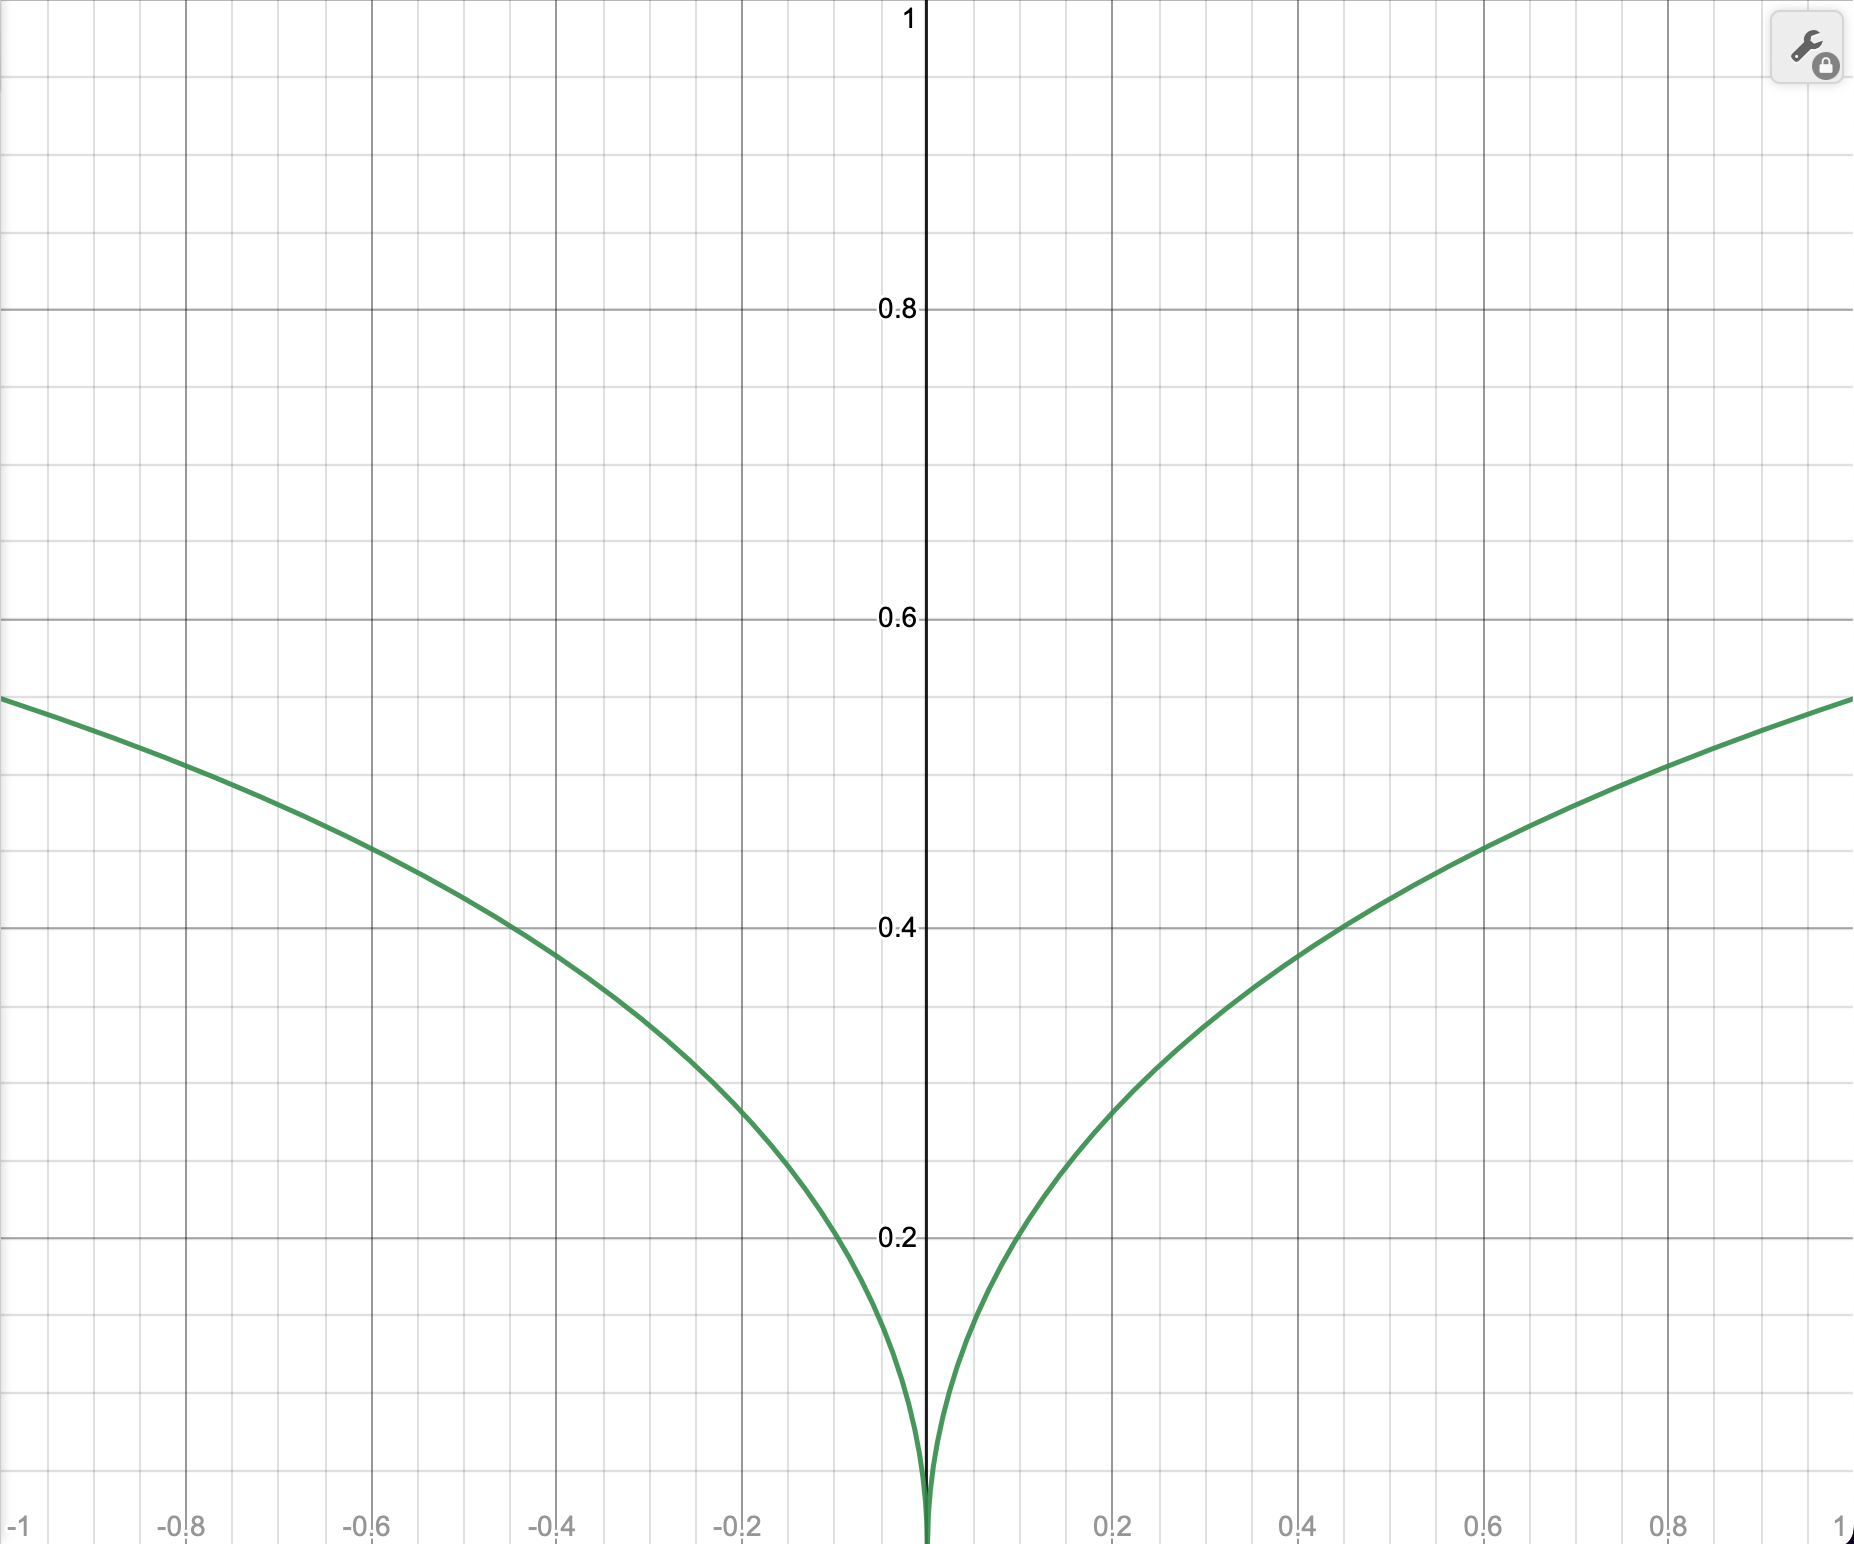
\includegraphics[width=8cm]{images/madFunction.png}
  \caption{Target Function}
  \end{figure}

It has a logarithmic behaviour and it's always positive, so $\log(|x|)$ is a good start. Since want the $x$ to assume values between 0 and 1, we have to normalize the distance by dividing it for 240, because it can take values between 0 and 240. Therefore we have also to add 1 inside the logarithm, otherwise the function will always give negative values.

\begin{figure} [!h]
  \centering
  \captionsetup{justification=centering}
  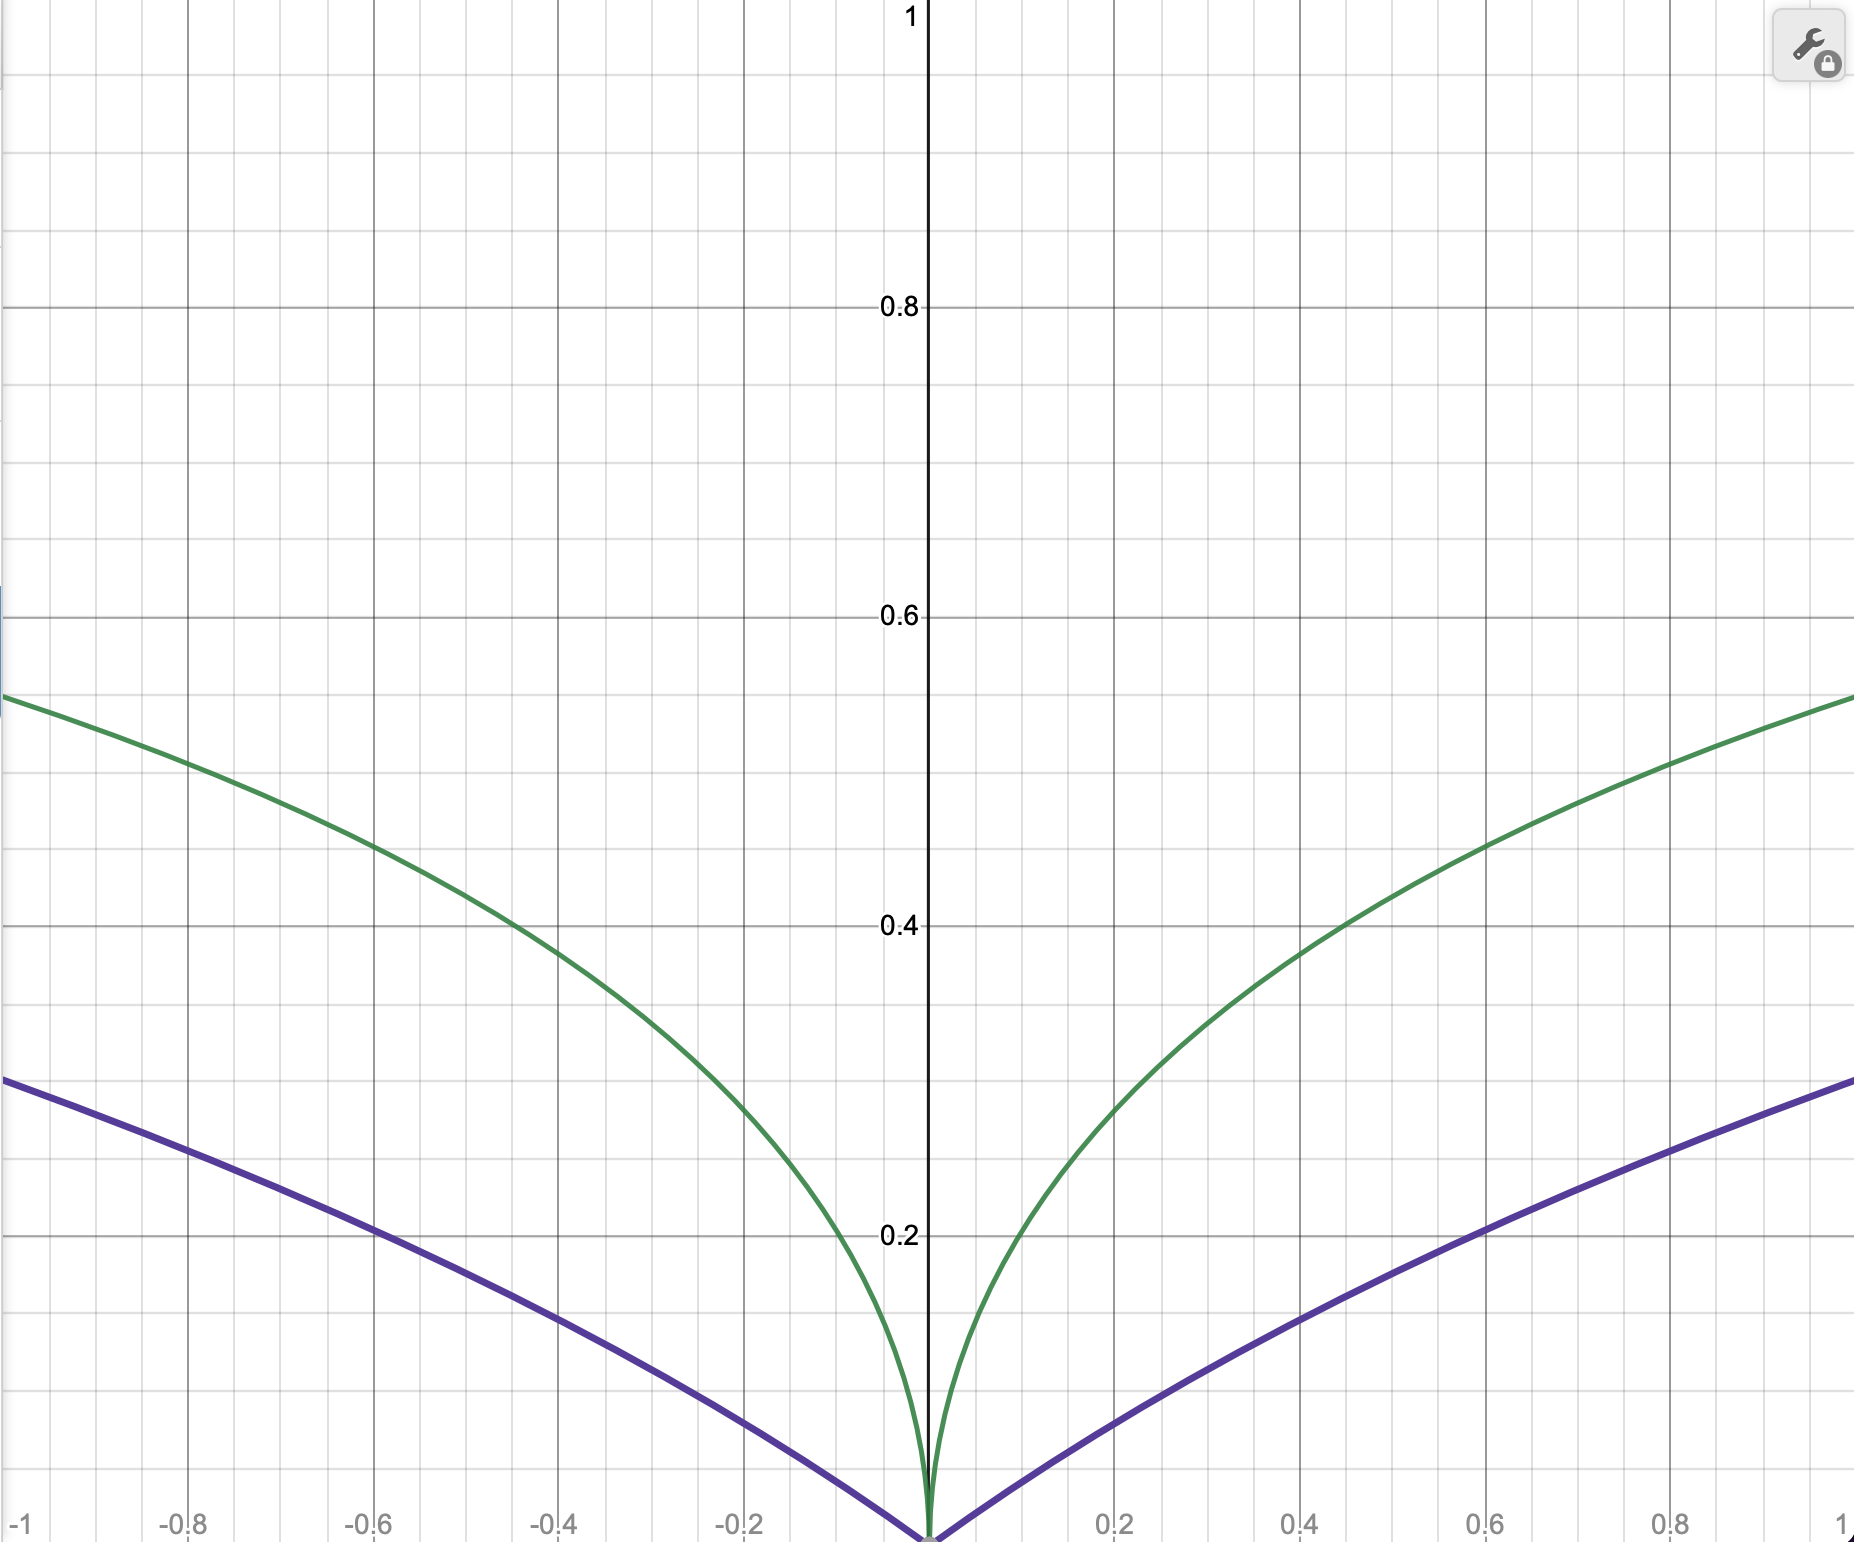
\includegraphics[width=8cm]{images/logx.png}
  \caption{${\color{violet}y=\log(|x|+1)}$ and ${\color{green}y=\sqrt{\log(|x|+1)}}$}
  \end{figure}

As you can see from the graph, its behaviour is too line-shaped to satisfy our goals. Thus we have to pump up the function. Since we are in the 0-1 range, we can't squared it, but we can square root it.
In practice, we also changed the scaling of the $x$ variable because we saw it worked better inside the range between the green and purple function.

\subsection{Hardware implementation}
Now we need to implement the function that acts on the robot.  

\subsection{How to recognize that the lane has ended}
To recognize the end of the track it's enough to just identify a stripe on the mid-bottom part of the warped image that has a huge amount of black pixels. This is because the warped image consider only the street immediately in front of the vehicle and thus if there is a road it will detect it with the corrispective amount of white pixels. To make the detection of the end of the lane more resistant to threshold's noise we will not check for the blackness of the full stripe but we will just make sure that there is at least the 95\% of black pixels on that region. \\
Moreover, even if small, there is a chance that the car can stop if we just detect blackness on just one frame. Thus, reasonably enough, we will take a mini-batch of frames and if most of them assess that the frames detected are black the car will simply stop or turn around.  

\subsection{How to turn around}
Once the end of the first round is detected, the car start turning back. The way it does that it's by giving a different power to the left and right motor. This allows the car to turn on itself till the camera detect the track again.\\

\section{Stop recognition using Haar Cascade Classifier}

\subsection{}

\subsection{}

\subsection{}

\subsection{Stop implementation in our car}


\section{Code}

The next code will be directly imported from a file (Random Code now)
\lstinputlisting[language=python]{../pedestrianDetection/StopDetection.py}


\section{Conclusion}
After designing the circuit required, assembling the circuit on the breadboard and having tested in multiple times with many test cases, we could build our autonomous vehicle which followed the white line track and switched mobility based on the claps from the environment just like a semi-autonomous vehicle! \\
\begin{figure}[!hbp]
\centering
  \begin{subfigure}[b]{0.4\textwidth}
  \centering
  \captionsetup{justification=centering}
    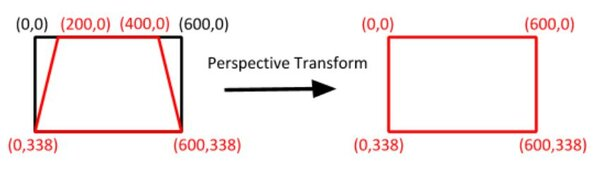
\includegraphics[width=\textwidth, height = 6cm]{images/perspective_transform.jpg}
    \caption{Front-Side view of chassis w/ circuit\\ (Redbot sensors attached)}
    \label{fig:g1}
  \end{subfigure}
  \hspace{1cm}
  \begin{subfigure}[b]{0.4\textwidth}
  \centering
  \captionsetup{justification=centering}
    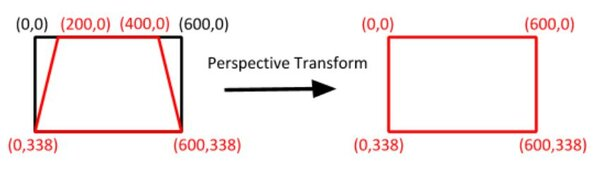
\includegraphics[width=\textwidth, height = 6cm]{images/perspective_transform.jpg}
    \caption{Side view of chassis \\(Motor, Arduino, Circuit visible)}
    \label{fig:g2}
  \end{subfigure}
  \caption{Photos of Final Lab Project}
\end{figure}

\section{Self-Evaluation $\&$ Future Projects}
We can say with utmost certainty that the takeaway from a project like this is definitely going to help in the future. Having designed an autonomous vehicles moving with cues from its environment we feel equipped with the tools to learn more about circuits and implement more complex circuits. Having learnt about using Microcontrollers, simple electrical components, microphones, and RedBot sensors, we are planning to take this project further by adding more sensors to improve and increase functionality. One idea for a future project is to add a heat sensor so that the car can move in a direction with a depression on the heat map - we plan on doing this using concepts of computer vision and machine learning to analyze the heat map and finding the minima on the map; a potential application of this is that the vehicle and autonomously change directions in case of a fire. Indeed, a project like this will be a great learning experience just like our final project was. \\

\subsection{Finding the curve}
We are at the core of our lane detection program. We have a black and white road seen from above and our car manage to drive in the center of the road. What we have to determine now is how do we find curves.\\
As I said before, we're going to determine it by summing the pixels on the y-axis. But how exactly are we going to do that? Well, we already found the center of the street, so we can imagine to draw a line passing through it. The side of the line that will have more white pixels determines the direction of the curve. But what about the intensity?\\
To get a grasp of what I mean imagine a frame of the road with a curve towards the left. If the curve is very round, then we will have a lot of white pixels in the left part of the curve. If it's not steep but just a small curve, then it will not have more many values on the left. Therefore, the idea is that the average x coordinate gives us the intensity of the curve. The computations are the same as the ones for the center of the street. How much curvy is a curve can be determined by summing the pixels in the columns of the whole image and taking only the non-noisy columns, as we did before. Then we can obtain, by subtracting this value to the one that represent the center of the road, the roundedness of the curve, that is represented by 


\section{References}
\begin{itemize}
\item[1] SparkFun - Flex Sensor\\ \url{https://cdn.sparkfun.com/datasheets/Sensors/ForceFlex/FLEXSENSORREVA1.pdf}
\item[2] ECE 110 - Experiment 9 - Navigation\\
\url{https://courses.engr.illinois.edu/ece110/fa2015/content/labs/Experiments/experiment.9.procedures.FA15.v10.pdf}
\item[3] RedBoard by SparkFun - Programmed with Arduino\\
\url{http://www.robotgear.com.au/Product.aspx/Details/733-RedBoard-by-SparkFun-Programmed-with-Arduino}
\item[4]  2N5192G ON Semiconductor | Mouser \\
\url{http://www.mouser.com/ProductDetail/ON-Semiconductor/2N5192G/?qs=vLkC5FC1VN$\%2Fa3d2jm7wSkw\%3D\%$3D}
\item[5] Sensors\\
\url{http://ixda.gatech.edu/resources/files/scott-sensors.pdf}
\item[6] Resistor - Wikipedia, the free encyclopedia\\
\url{https://en.wikipedia.org/wiki/Resistor}
\item[7] Capacitor - Wikipedia, the free encyclopedia\\
\url{https://en.wikipedia.org/wiki/Capacitor}
\item[8] Ceramic Capacitor $>>$ Capacitor Guide\\
http://www.capacitorguide.com/ceramic-capacitor/
\item[9] Transistor - Wikipedia, the free encyclopedia\\
\url{https://en.wikipedia.org/wiki/Transistor}
\end{itemize}

\noindent\rule{18.5cm}{0.4pt}
\end{large} 
\end{document}